\section{Einleitung}

\begin{frame}
	\frametitle{Aktuelle Nachrichten}
	\only<1>{
		\begin{figure}
		\centering
		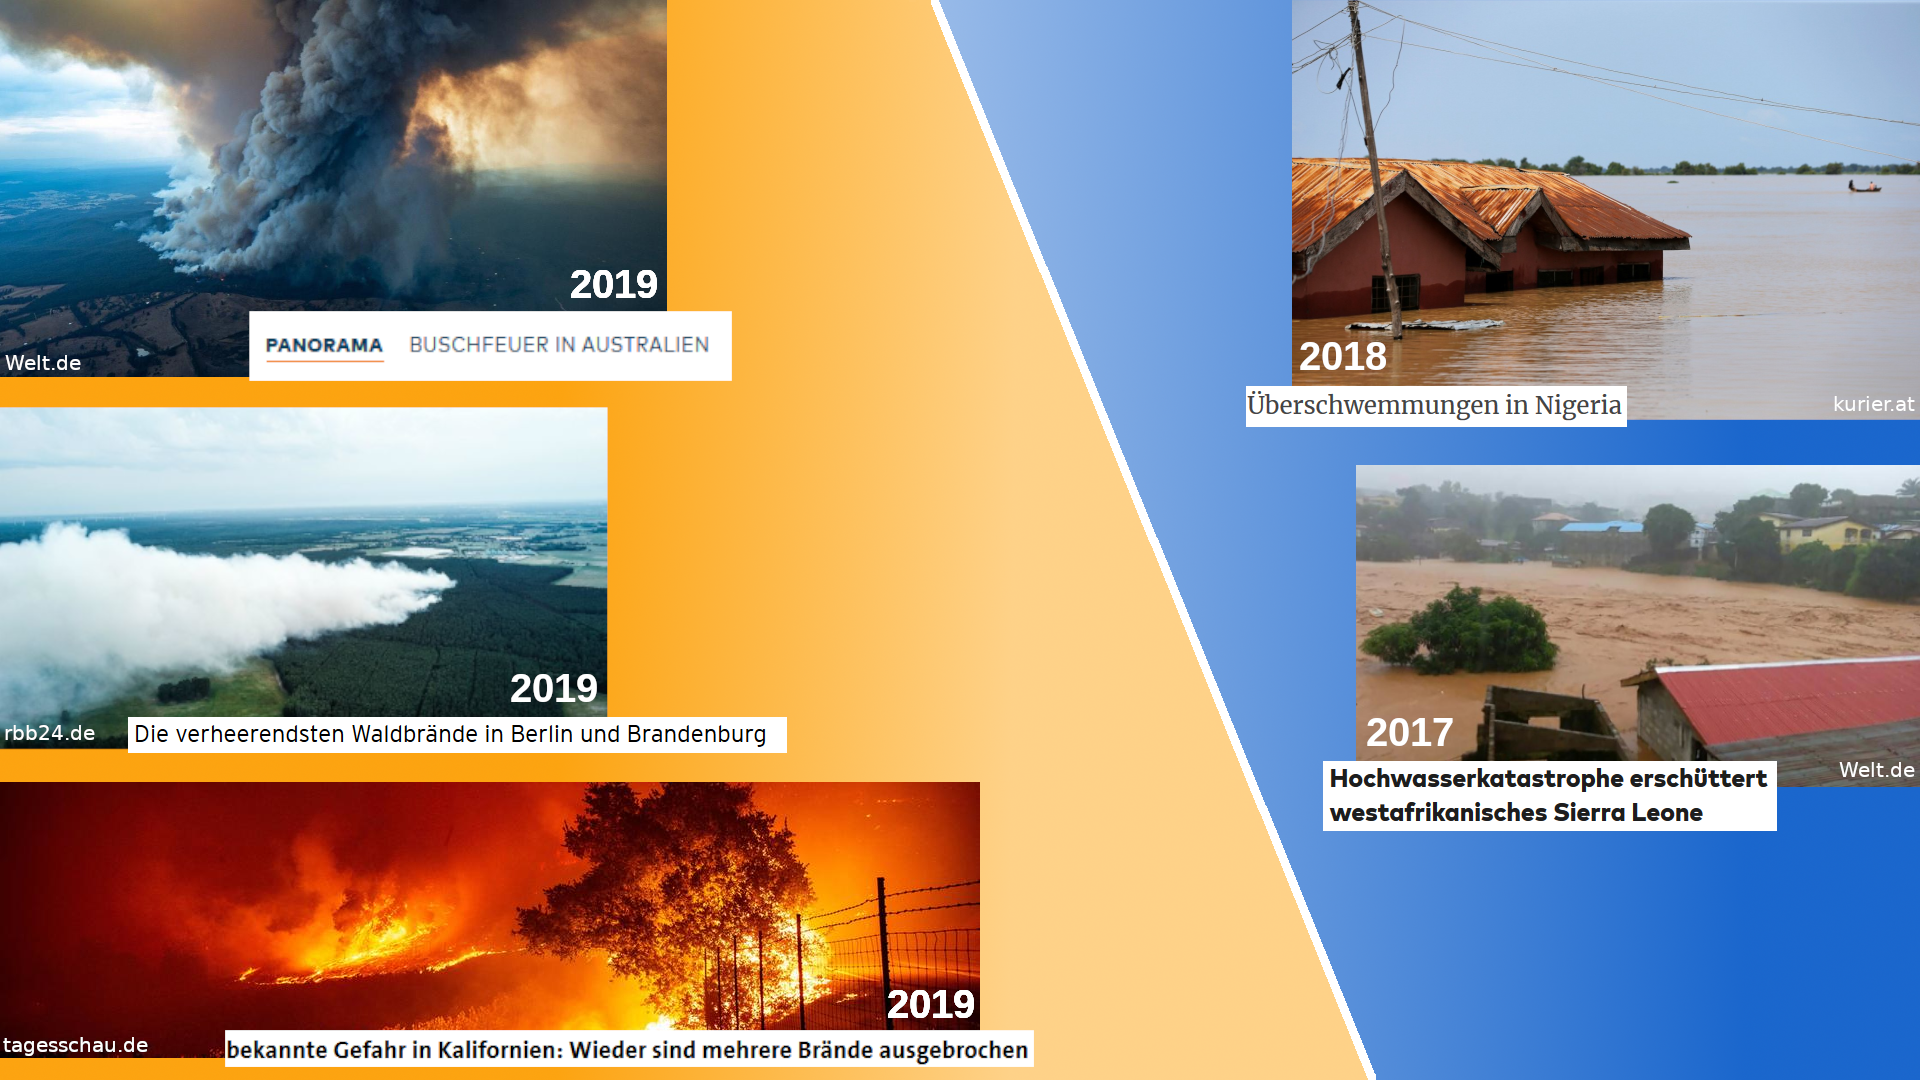
\includegraphics[width=0.9\linewidth]{bilder/CurrentSituation}
		\end{figure}

		\note{
			Wetterereignisse der letzten drei Jahre
			\begin{itemize}
				\item[2017] Hochwasserkatastrophe in Sierra Leone durch bis du dreifach höheren Regenfall als üblich, keine Unwetterwarnung der Regierung, unkontrollierte Entwaldung, Müllverstopfte Kanalisation, etc.
				\item[2018] Überschwemmungen in Nigeria und vielen anderen afrikanischen Ländern, mehrere Millionen Menschen obdachlos
				\item[2019] Buschbrände in Kalifornien, mehr als \SI{1000}{km\squared} (etwa drei mal die Fläche von Dortmund) verbrannt, gehört zu den größten 5 Buschbränden. 4 der größten 5 in den letzten 10 Jahren
				\item[2019] Waldbrände in Brandenburg, größte Waldbrände der Geschichte des Landes (etwa 1,5 mal größer als bisher größter),
				etwa \SI{7,50}{km\squared} (etwa die Fläche von Dorstfeld) verbrannt.
				\item[2019] Buschfeuer in Australien, \SI{186000}{km\squared} (\nicefrac{1}{2} mal die Fläche von Deutschland) verbrannt, etwa 1 Mrd. Tiere getötet, Rauch auch in Argentinien und Chile spührbar, wird Black Summer genannt.
			\end{itemize}
		}
	}
	\only<2>{
	\begin{figure}
		\centering
		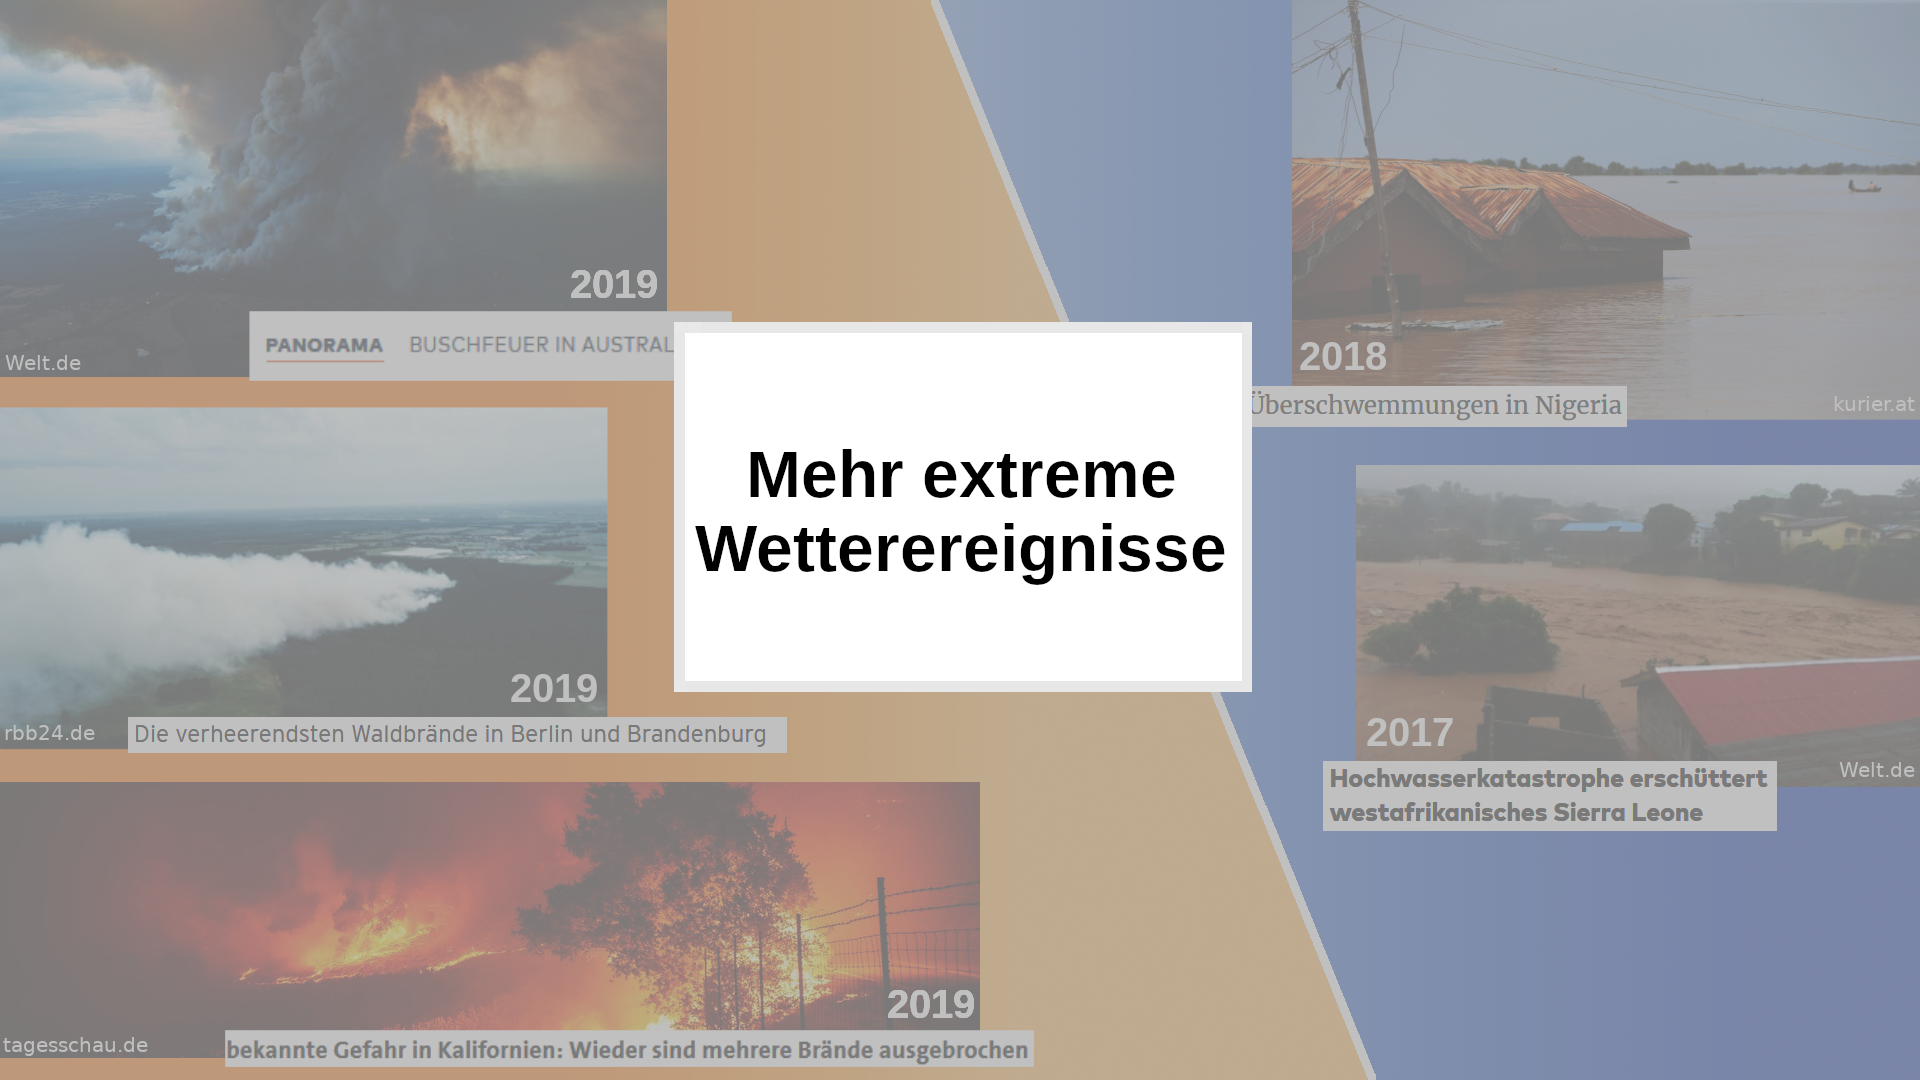
\includegraphics[width=0.9\linewidth]{bilder/CurrentSituation_Conclusion}
	\end{figure}
	}
	\only<3>{
	\begin{figure}
		\centering
		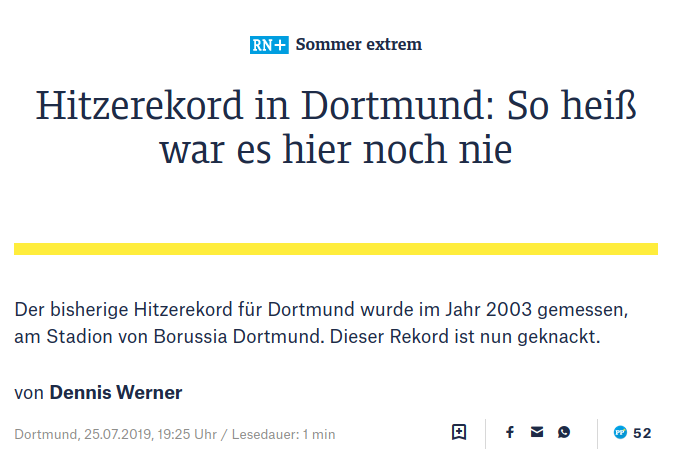
\includegraphics[width=0.5\linewidth]{bilder/dortmund}
	\end{figure}
	\begin{center}
		\textbf{Auch bei uns}
	\end{center}
	\note{
		Man muss gar nicht so weit gehen, in Dortmund ist es genau so
	}
	}

\end{frame}

% "es war doch immer schon im Sommer warm"


\begin{frame}
	\frametitle{Warming Stripes}
	% Abbildung der Warming Stripes: Die Entwicklung ist wirklich dramatisch

	% Farbskala erklären
	\begin{figure}
		\centering
		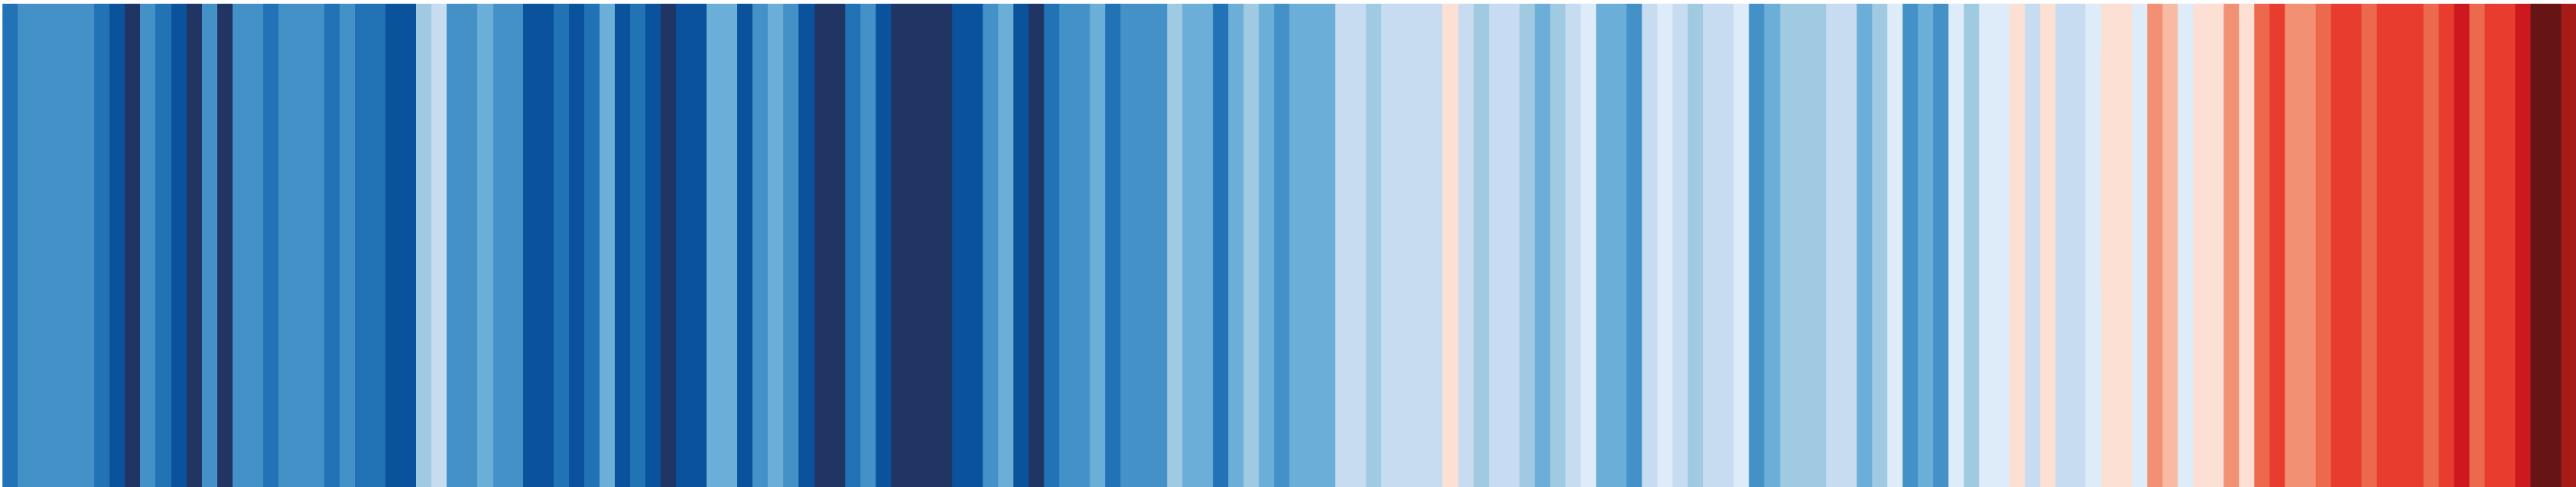
\includegraphics[width=\linewidth]{bilder/s4f-warming-stripes}
		\caption{Die \textit{Warming Stripes}}
		\label{fig:s4f-warming-stripes}
	\end{figure}
	\begin{itemize}
		\item Jeder Balken repräsentiert eine Jahr aus der Periode 1850-2017
		\item Blau = kälter als der Mittelwert, Rot=Wärmer
		\item Je dunklere die Farbe, desto extremer die Abweichung vom Mittelwert
		\item Die Trend geht klar zu höheren Temperaturen
		\item Übrigens auch das Logo der Scientists 4 Future \url{https://scientists4future-dortmund.de/}
	\end{itemize}

	\note{
	\begin{itemize}
		\item[] Global zusammenfassen für ein Großteil der verfügbaren Temperaturdaten
		\item[] Warming stripes, Logo der S4F
		\item[] Jeder Balken Jahresmittelwert globaler Luft- und Wassertemperaturen
		\item[] Wer Interesse an den Daten hat, kann sich das auf unserer Homepage noch einmal genau anschauen
	\end{itemize}
	}
\end{frame}

\begin{frame}
	\frametitle{Warming Stripes}
	% Extrapolation der Warming Stripes
	\begin{figure}
		\centering
		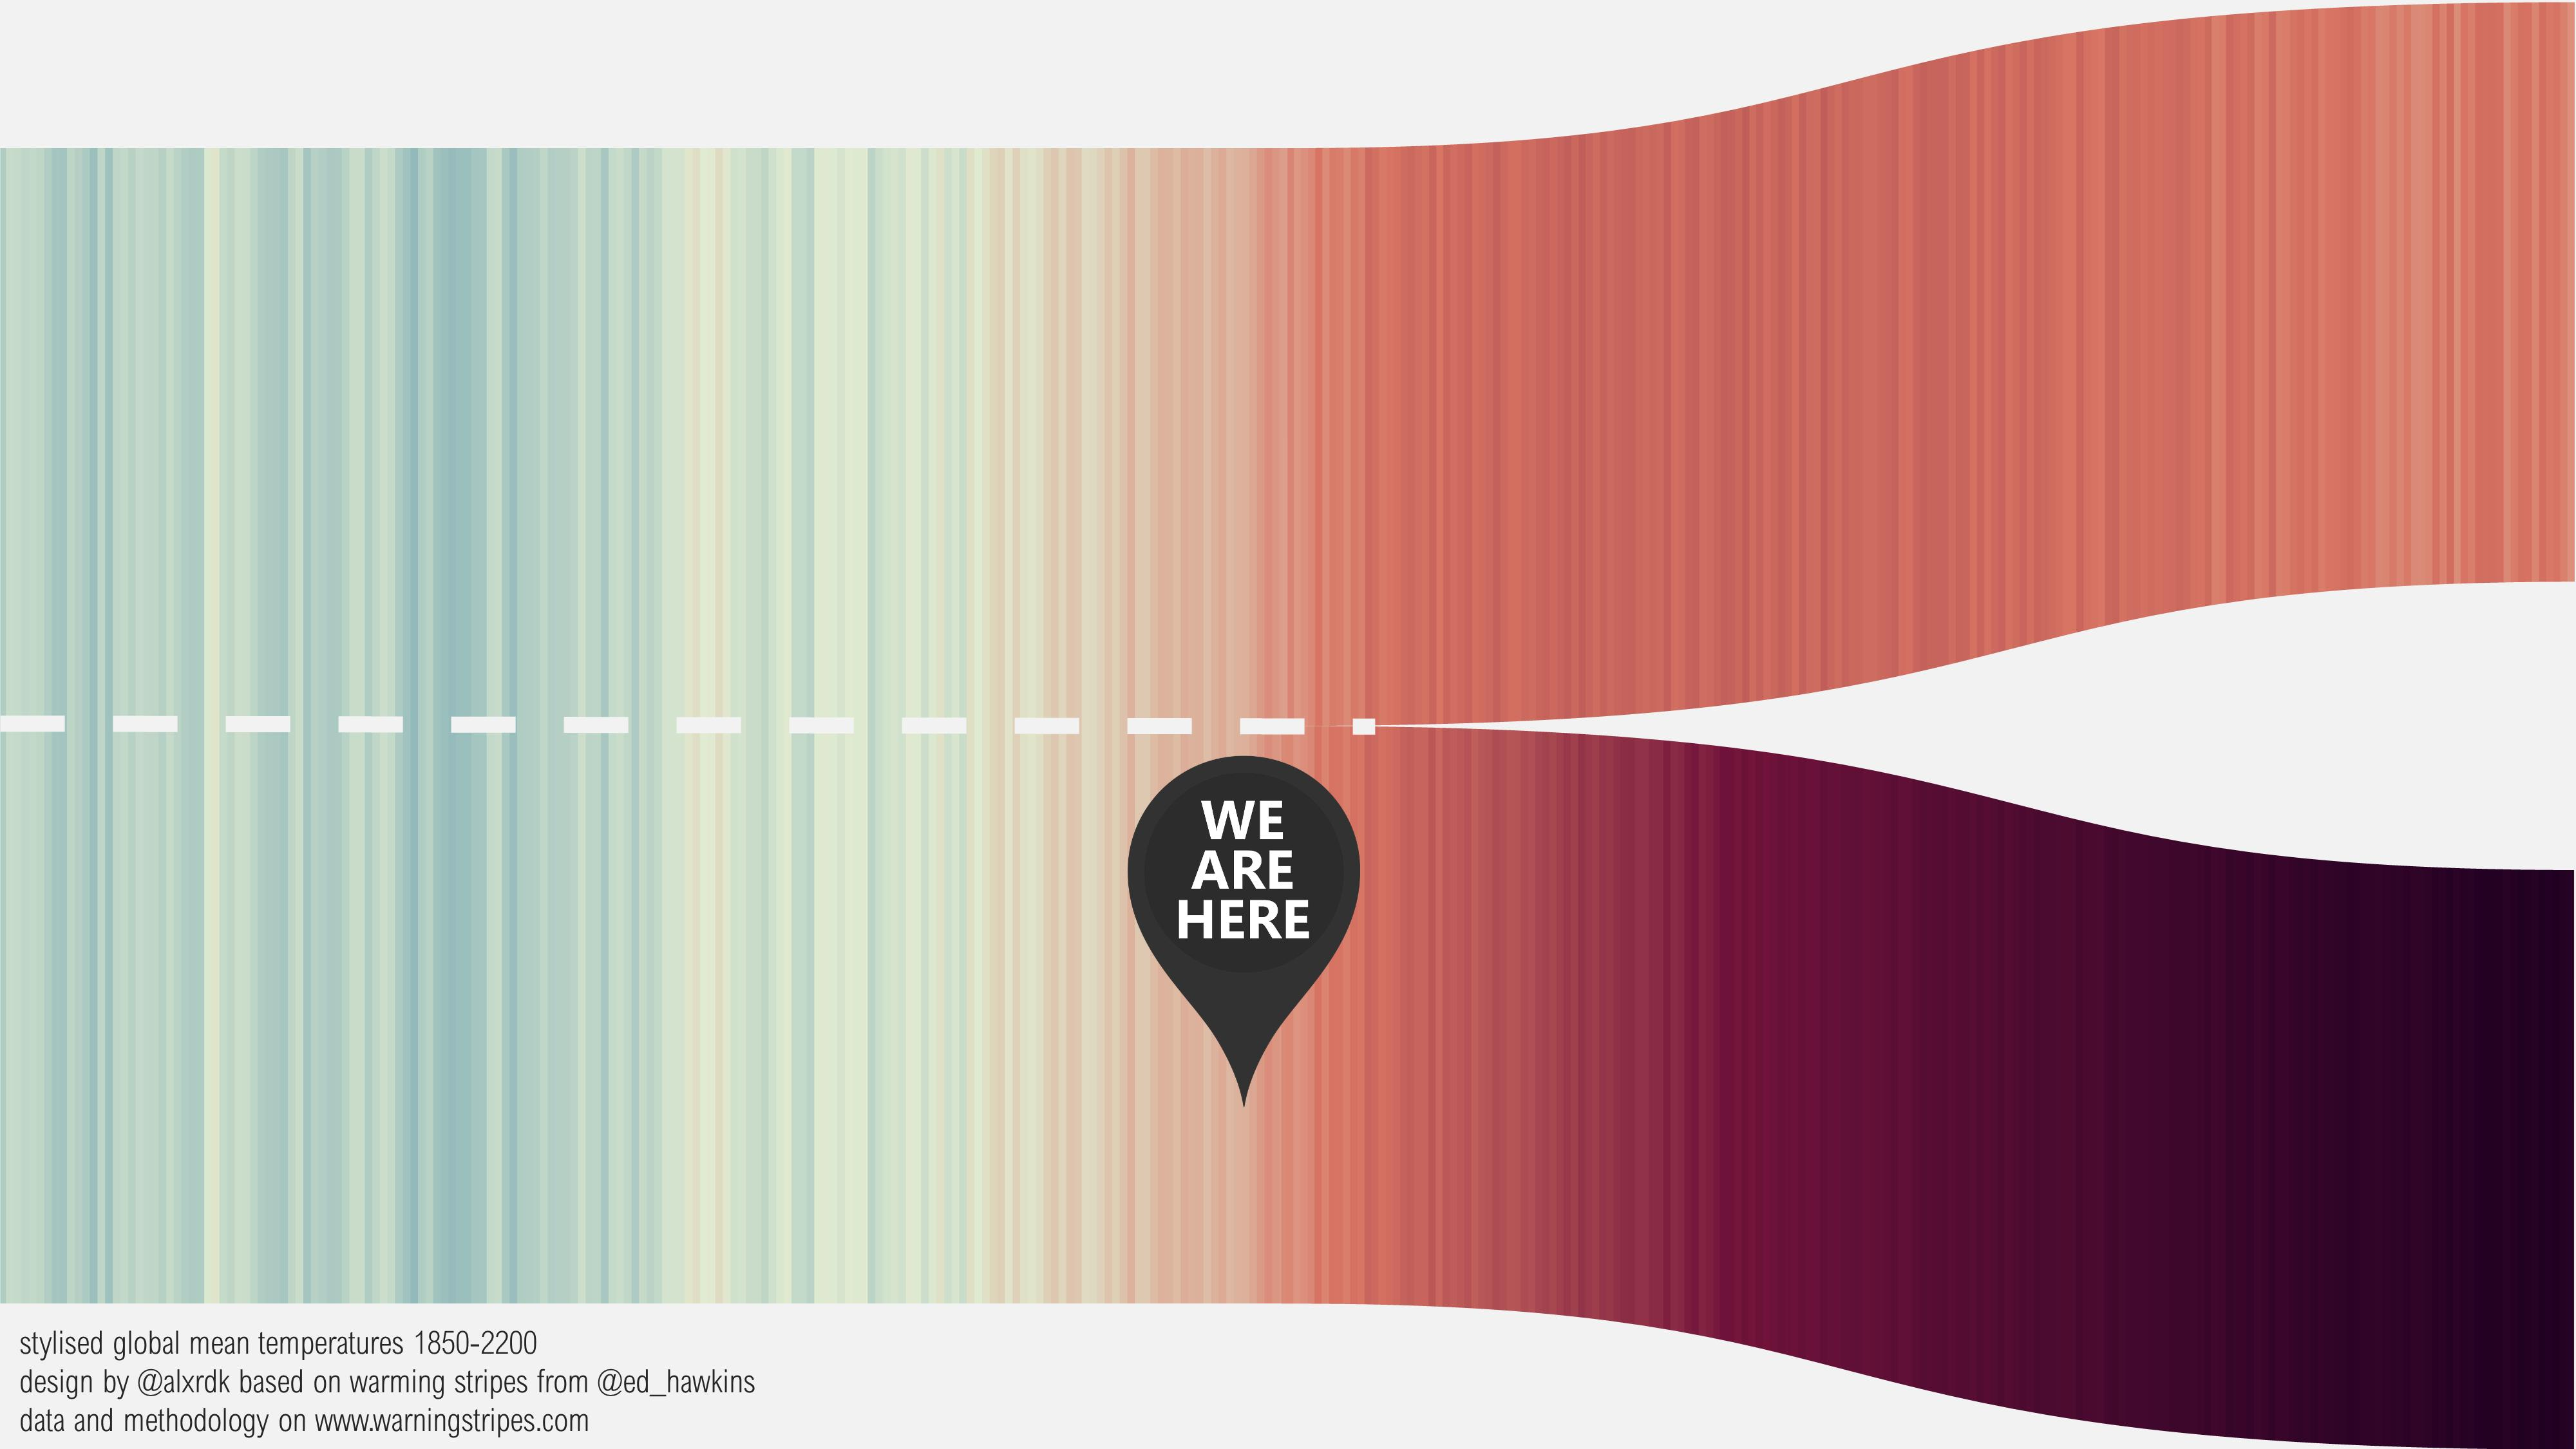
\includegraphics[width=0.55\linewidth]{bilder/warming_stripes_zukunft}
		\caption{Extrapolation der \textit{Warming Stripes} basierend auf Modellannahmen}
	\end{figure}
	\begin{itemize}
		\item In der Zukunft wird es sehr wahrscheinlich zu einer weiteren Erwärmung kommen
		\item Man kann statistische Prognosen für die Zukunft auf Basis von Modellrechnungen erstellen
		\item Der genaue Trend und die maximale Erwärmung hängen aber davon ab was wir heute und in den nächsten Jahren tun!
	\end{itemize}

\end{frame}
